\documentclass[border=10pt]{standalone}
\usepackage{pgfplots}
\pgfplotsset{compat=1.18}
\begin{document}
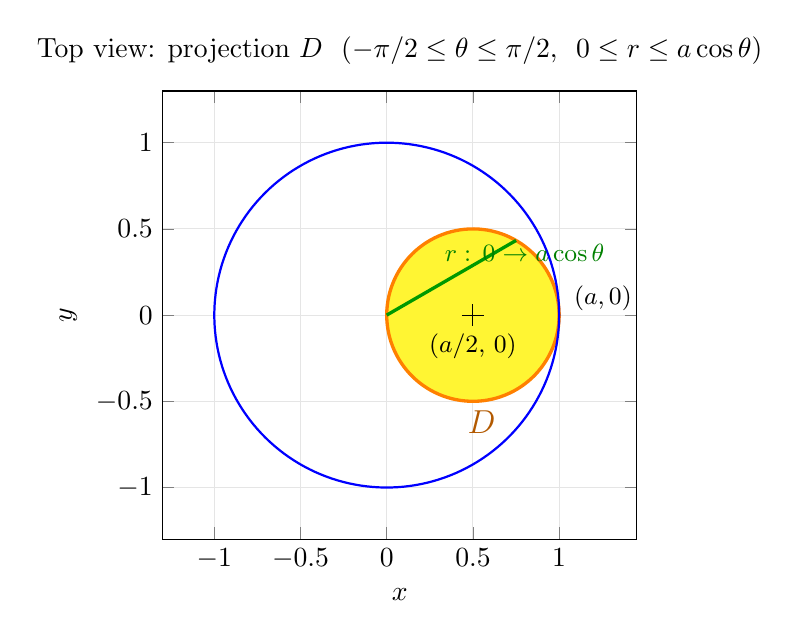
\begin{tikzpicture}
\begin{axis}[
    axis equal image,
    xlabel={$x$}, ylabel={$y$},
    xmin=-1.3, xmax=1.45, ymin=-1.3, ymax=1.3,
    title={Top view: projection $D$ \ ($-\pi/2 \leq \theta \leq \pi/2$, \ $0 \leq r \leq a\cos\theta$)},
    grid=both, grid style={gray!20}]
% shaded region D = half-disk bounded by circle r=a cos(theta) and the y-axis
\addplot[fill=yellow!80, draw=orange, very thick, domain=-90:90, samples=120]
    ({cos(x)^2}, {cos(x)*sin(x)}) \closedcycle;
% sphere footprint
\addplot[blue, thick, domain=0:360, samples=180]
    ({cos(x)}, {sin(x)});
% ray r: 0 -> a cos(theta) at theta = 30 degrees
\addplot[green!60!black, very thick, domain=0:cos(30), samples=2]
    ({x*cos(30)}, {x*sin(30)});
% center of cylinder
\addplot[only marks, mark=+, mark size=4, black] coordinates {(0.5,0)};
\node[anchor=north] at (axis cs:0.5,-0.05) {\small $(a/2,\,0)$};
\node[anchor=west] at (axis cs:1.03,0.1) {\small $(a,0)$};
\node at (axis cs:0.55,-0.62) {\large $\color{orange!70!black}D$};
\node[anchor=west] at (axis cs:0.28,0.36) {\small $\color{green!50!black}r:\,0 \to a\cos\theta$};
\end{axis}
\end{tikzpicture}
\end{document}